\chapter{User Interface Design}
\label{chap:user-interface-design}%

\par This section presents the User Interface (UI) and User Experience (UX) design of
the Best Bike Paths (BBP) system. Since BBP is primarily a mobile-based application,
the interface is designed following a mobile-first approach, taking into account the
constraints and interaction patterns of smartphone usage. The goal of the UI/UX
design is to enable users to access the system’s functionalities in a simple, safe,
and efficient manner, even in contexts where attention and interaction time may be
limited.

\par The design emphasizes clarity, consistency, and ease of navigation. Screens are
structured to minimize cognitive load and to present only the most relevant
information at each step of the user interaction. Actions commonly performed while
cycling, as well as shortly before and after a trip, are designed to require a minimal
number of gestures and to provide immediate and clear feedback.

\par The interface is illustrated through a set of mobile application mockups created
using Figma as a design tool. These mockups follow the main user flows of the system
and represent the expected layout and functional organization of the application.
They are used to explain how users interact with BBP during typical usage scenarios.
Separate interaction flows are described for different user types, reflecting the
distinction between registered and unregistered users defined in the RASD.

\par For the sake of clarity, not all application screens are shown. Simple or
self-explanatory views, as well as screens that closely resemble others in structure
or behavior, are omitted from the document. When this occurs, the missing steps in
the user flow are briefly described in text to preserve continuity and completeness.

\par The included screenshots correspond to a mockup version of the mobile application
developed in Figma and are intended to represent the structural and functional aspects
of the interface. They do not define the final graphical style of the system and may
omit or simplify specific visual elements such as colors, icons, and detailed
graphics. These aspects are intentionally abstracted in order to focus on interaction
flow, layout, and usability, which are the primary concerns at this stage of the
design.


\section{User Flow Diagram}
\label{sec:user-flow-unified}

\begin{figure}[H]
    \centering
    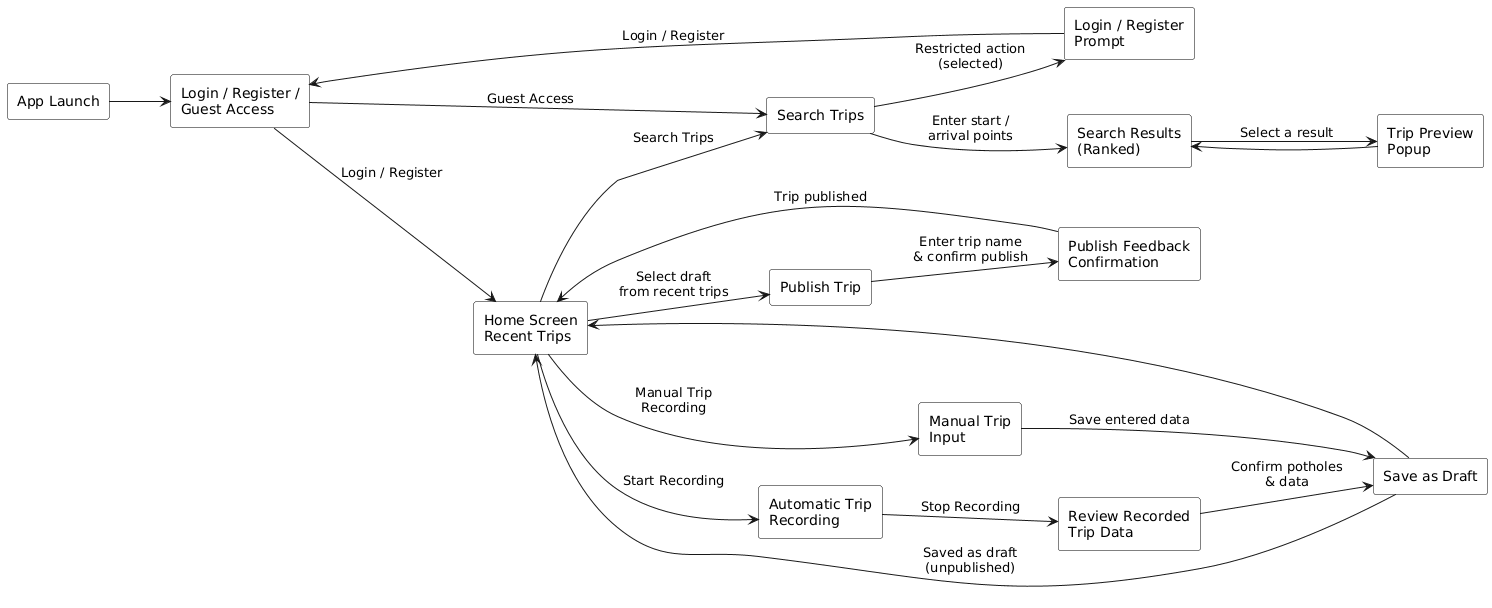
\includegraphics[width=0.98\textwidth]{Images/RV_SRC/user_flow_diagram.png}
    \caption{Unified User Flow Diagram for the BBP Mobile Application}
    \label{fig:bbp-user-flow-diagram}
\end{figure}

\par Figure~\ref{fig:bbp-user-flow-diagram} illustrates the unified user flow of the
Best Bike Paths (BBP) mobile application, capturing the main interaction paths for
both registered cyclists and unregistered users (guests). The diagram highlights
how users navigate through the application starting from the initial access screen,
and how available functionalities differ based on authentication status.

\par Upon launching the application, users are presented with an initial screen that
allows them to either log in, register a new account, or continue as a guest. Users
who authenticate or register successfully are redirected to the Home Screen, which
serves as the central hub of the application. From this screen, registered cyclists
can access the core functionalities of BBP, including automatic trip recording,
manual trip data entry, and trip search.

\par When starting an automatic recording session, the user can stop the recording
at any time and is redirected to a review screen where collected data is displayed.
At this stage, the cyclist can validate detected events, such as potholes, and save
the trip as a draft. Draft trips appear in the Home Screen under recent trips and can
be further edited or published. Publishing a trip requires explicit confirmation,
including the insertion of a trip name, and provides clear feedback upon completion
of the action.

\par Manual trip recording follows a similar workflow, allowing users to insert trip
data directly without automatic tracking. Manually entered trips are also saved as
drafts and can be published at a later time through the same confirmation process.

\par Both registered and unregistered users can access the trip search functionality.
Users may specify a starting point and a destination to retrieve a ranked list of
available trips. Selecting a result displays a brief preview with summarized
information about the trip. This interaction remains read-only for unregistered
users.

\par Guest users are intentionally limited to browsing and searching for trips. Any
attempt to access restricted functionalities, such as trip recording, draft
management, or publishing, triggers a prompt inviting the user to log in or register.
This mechanism ensures a smooth transition from guest usage to full account creation
while preserving a low-friction initial experience.


\subsection{Login}
\label{subsec:login}%

\begin{figure}[H]
    \centering
    \begin{minipage}{0.48\textwidth}
        \centering
        \fbox{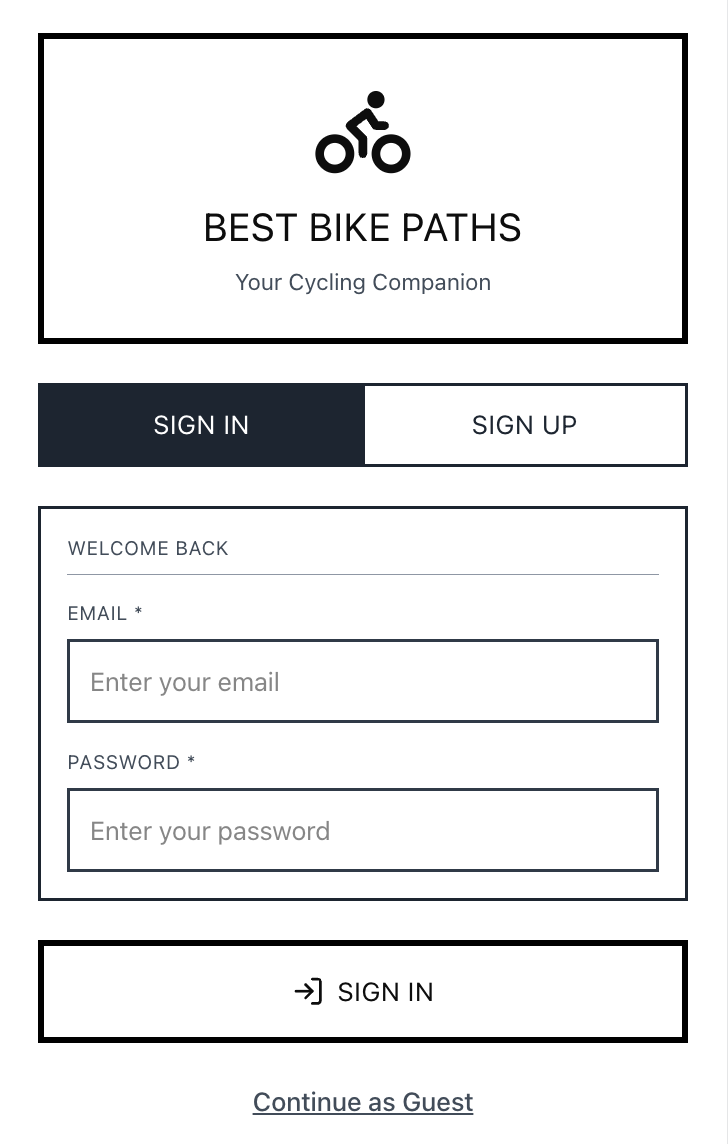
\includegraphics[width=\textwidth]{Images/RV_SRC/BBP_UI/signin.png}}
        \caption{Login Page - ST}
        \label{fig:login-page-st}
    \end{minipage}
    \hfill
    \begin{minipage}{0.48\textwidth}
        \centering
        \fbox{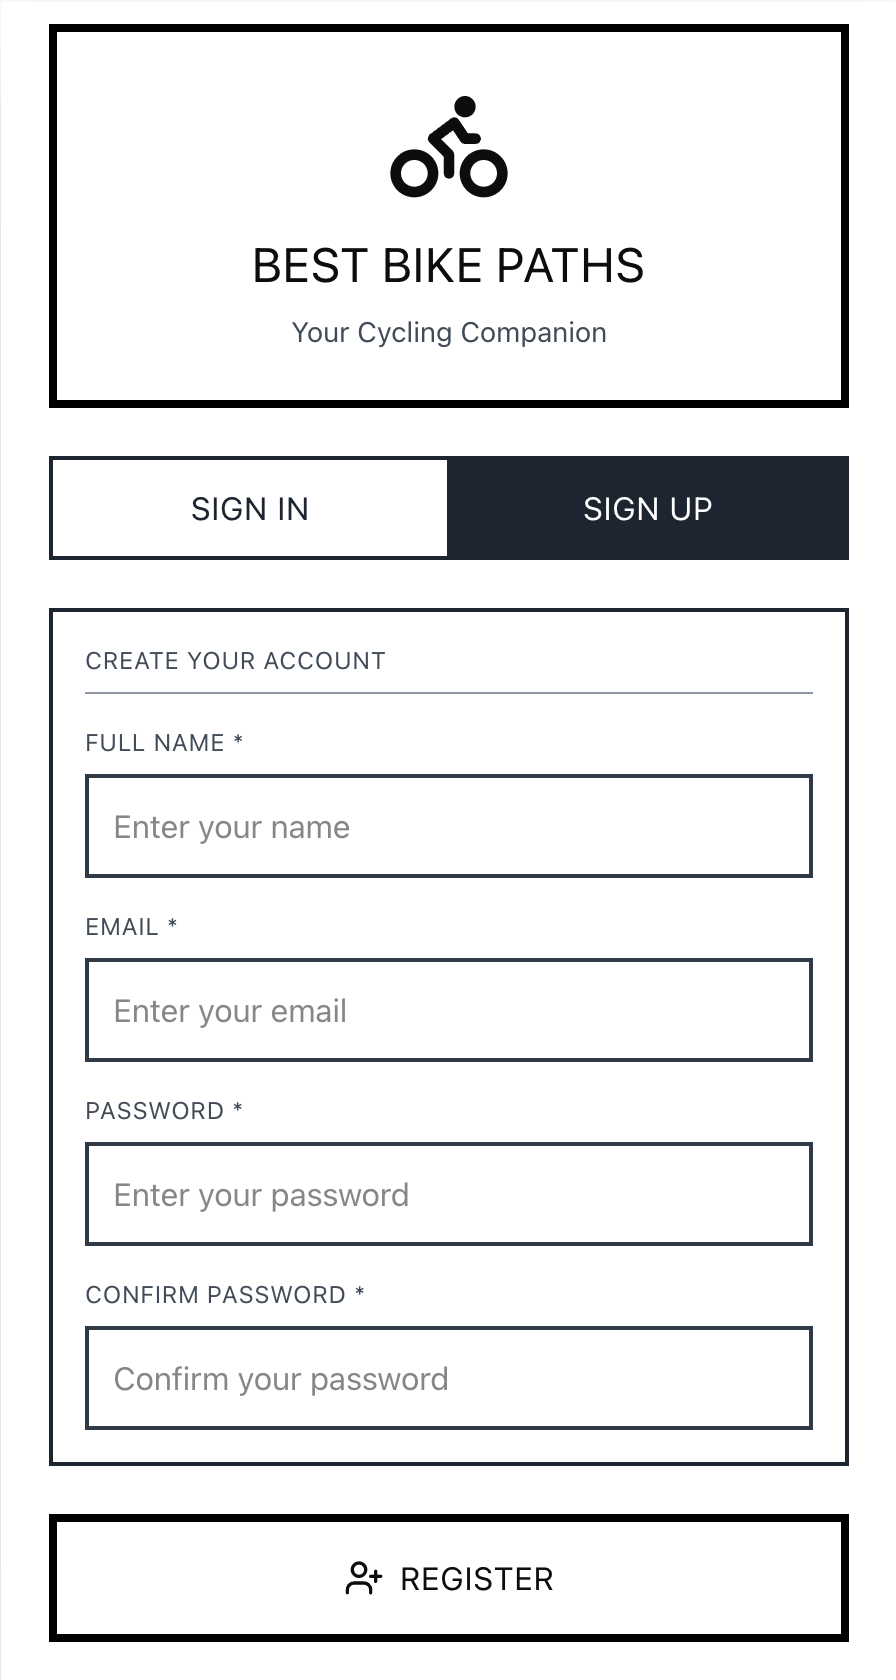
\includegraphics[width=\textwidth]{Images/RV_SRC/BBP_UI/signup.png}}
        \caption{Signup Page - ST}
        \label{fig:signup-page-st}
    \end{minipage}
\end{figure}

\par The BBP login page serves as the initial entry point for the platform. Users are presented with three primary options: they can authenticate using previously created credentials, register a new account by providing their name, email, and password, or choose to "Continue as Guest." This final option allows unregistered users to immediately access the public map and navigation features without authentication, satisfying the requirement for open access to the bike path app.
\subsection{User Profile}
\label{sect:user_profile}

\begin{figure}[H]
    \centering
    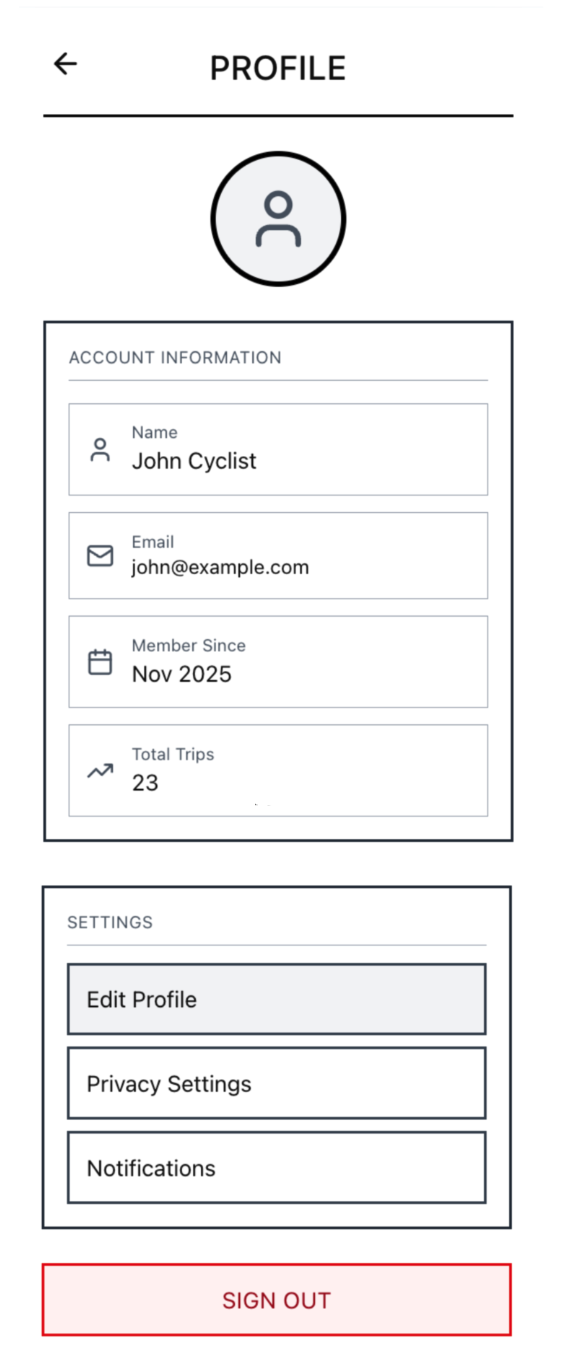
\includegraphics[height=0.8\textheight, keepaspectratio]{Images/RV_SRC/BBP_UI/profilescreen.png}
    \caption{Mockup of the BBP User Profile UI}
    \label{fig:user_profile}
\end{figure}

\par The Profile interface is accessible via the user icon located in the global header. It serves as the central hub for managing the registered user's account details and preferences. The upper panel, "Account Information," identifies the user and displays key membership details. Notably, it includes a "Total Trips" counter, which provides a high-level summary of the user's engagement, consistent with the system's requirement to store and track cycling activities over time.

\par The lower section focuses on account configuration. The "Settings" menu allows users to modify their personal details via "Edit Profile" and manage application preferences such as "Notifications." Crucially, the "Privacy Settings" option is available to control data visibility, which is particularly relevant given that users can choose to publish or keep their trip data private. Finally, a prominent "Sign Out" button at the bottom ensures users can securely terminate their session.
\subsection{Homepage}
\label{sect:homepage}

\begin{figure}[H]
    \centering
    % Limits height to 45% of the page text height to fit vertically
    % keepaspectratio ensures the image doesn't get distorted
    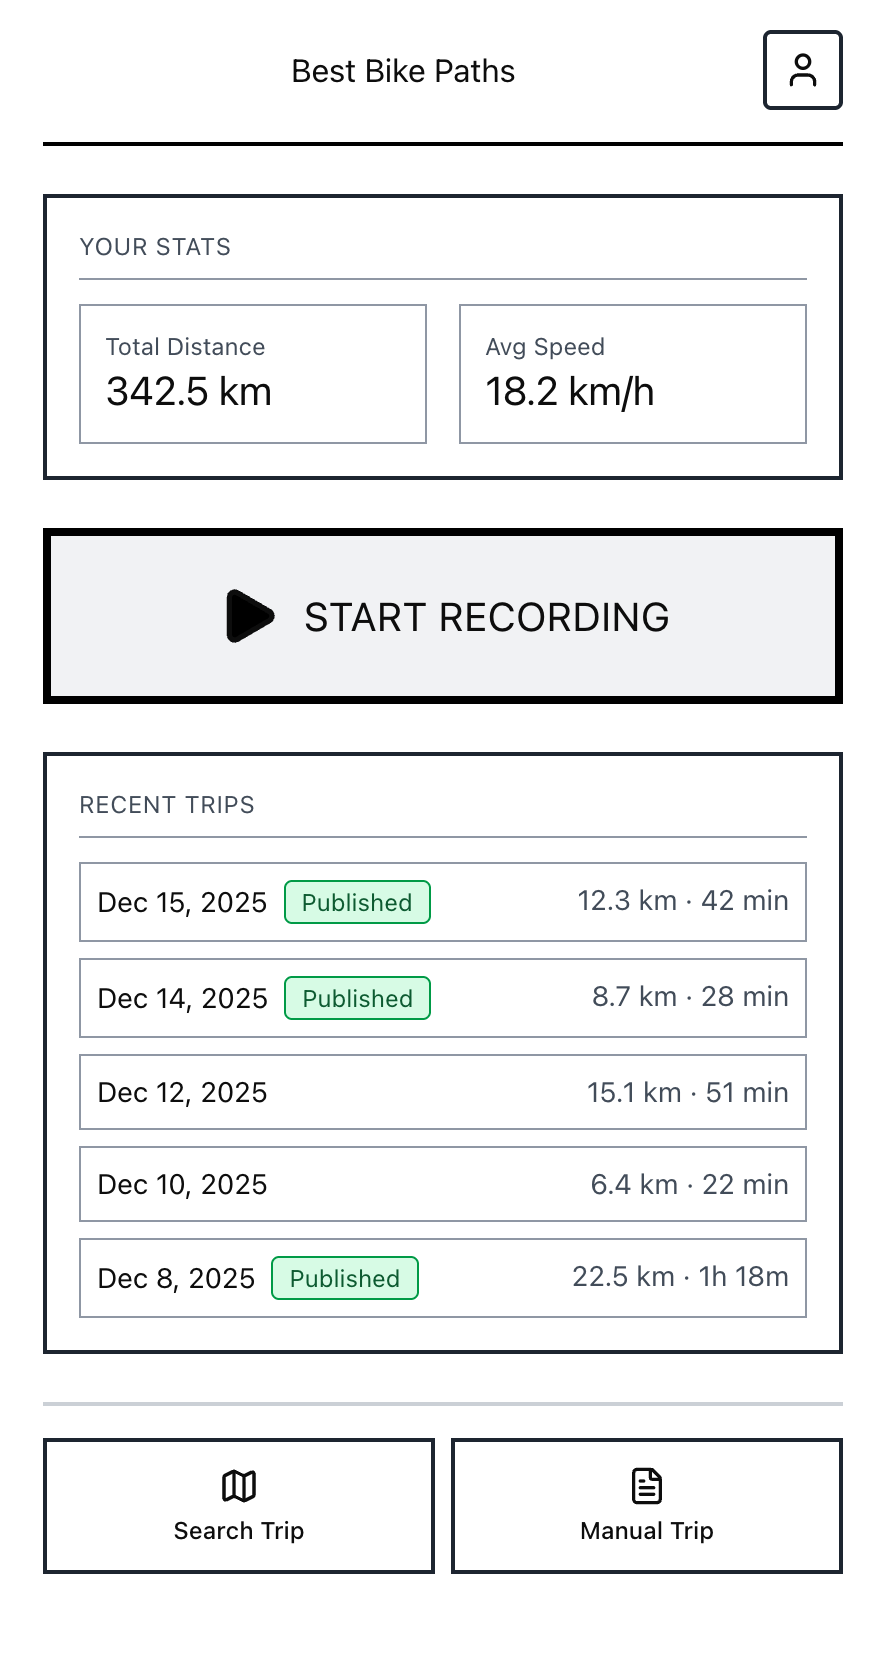
\includegraphics[height=0.8\textheight, keepaspectratio]{Images/RV_SRC/BBP_UI/homepage.png}
    \caption{Mockup of the BBP Homepage UI}
    \label{fig:homepage}
\end{figure}

\par The homepage is the main entry point for the BBP application. Here the user can view a summary of their cycling performance, specifically their total distance covered and average speed. As with all other pages, the header is present and allows the user to access their profile to manage personal settings or log out.

\par The central section features a prominent "Start Recording" button, enabling the user to instantly initiate the \textit{Automated Mode}, where the system acquires data from the mobile device sensors while biking. Below the main action area, a "Recent Trips" section lists the user's history, displaying key details such as date, distance, duration, and the publication status (e.g., "Published") for each trip. Finally, the footer navigation provides quick access to two other core functionalities: "Search Trip," allowing users to visualize bike paths on a map between an origin and destination, and "Manual Trip," which enables the manual insertion of trip data and path status.

\subsection{Auto Recording Trip Interface}
\label{sect:auto_recording_trip}

\begin{figure}[H]
    \centering
    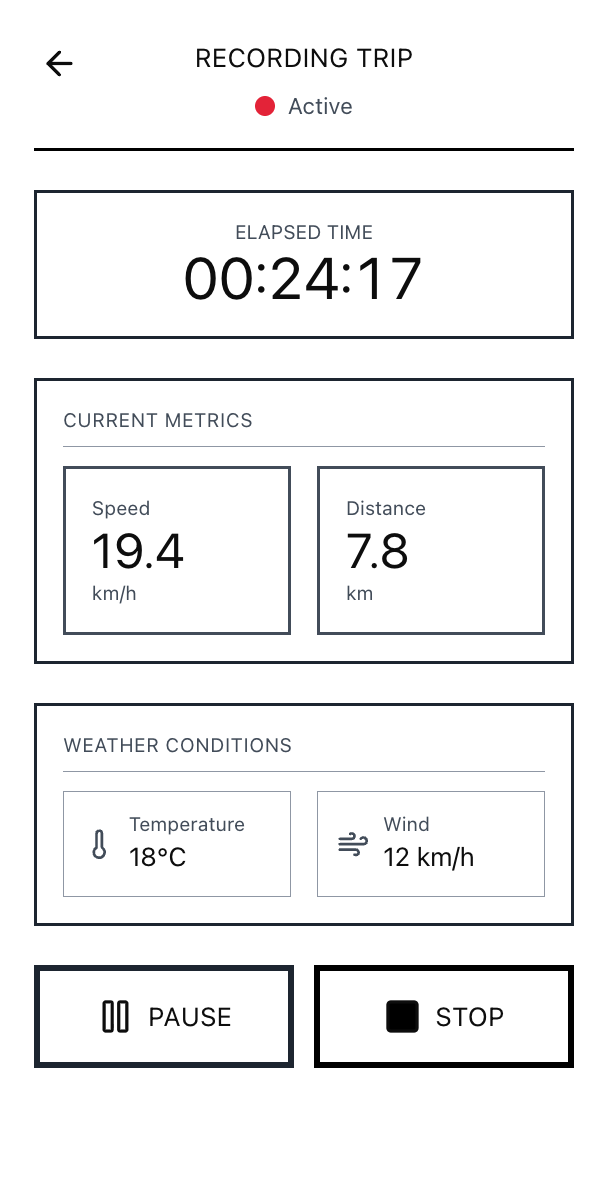
\includegraphics[height=0.6\textheight, keepaspectratio]{Images/RV_SRC/BBP_UI/autorecord.png}
    \caption{BBP Auto Recording Trip UI}
    \label{fig:auto:recording_trip}
\end{figure}

\par This interface is activated immediately after the user selects "Start Recording" from the homepage. It represents the active state of the \textit{Automated Mode}, providing the user with real-time monitoring of their current activity. A status indicator at the top confirms that the system is actively tracking the session.

\par The central dashboard is divided into three key informational areas. The top section displays the "Elapsed Time" since the start of the trip. Below this, the "Current Metrics" panel provides live feedback on the user's performance, specifically showing the current speed and the total distance covered so far, derived from the device's GPS and sensor data.

\par Additionally, the application enriches the trip context through the "Weather Conditions" panel. As specified in the system requirements, this section displays real-time meteorological data, such as temperature and wind speed, retrieved from external services. Finally, the footer offers "Pause" and "Stop" controls, allowing the user to manage the recording session. Pressing "Stop" will conclude the data acquisition and proceed to the verification stage where the user can confirm the reconstructed path.

\subsection{Trip Completion and Verification}
\label{sect:trip_complete}

\begin{figure}[H]
    \centering
    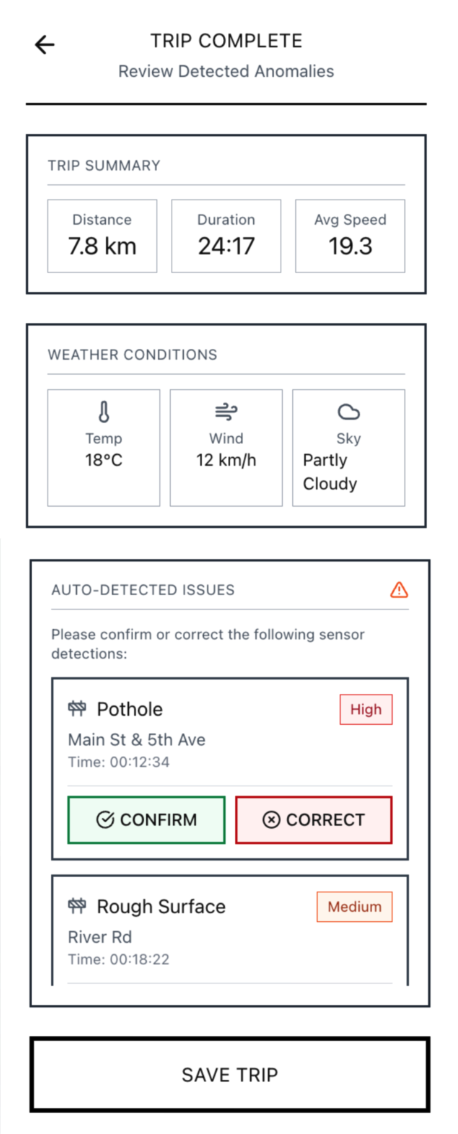
\includegraphics[height=0.9\textheight, keepaspectratio]{Images/RV_SRC/BBP_UI/autotripcomplete.png}
    \caption{Summary and Anomaly Verification UI}
    \label{fig:trip_complete}
\end{figure}

\par Upon stopping the recording, the user is presented with the Trip Complete interface. The top section provides a "Trip Summary" containing the final statistics, total distance, duration, and average speed, recorded during the session. Consistent with the recording interface, the final meteorological conditions are also displayed to provide context to the performance metrics.

\par The core feature of this screen is the "Auto-Detected Issues" panel, which addresses the requirement for validating sensor data. As the system automatically detects anomalies (such as potholes or rough surfaces) using the device's accelerometer and gyroscope during the ride, they are listed here for user review. To mitigate potential false positives, the user is required to interact with each detected item by selecting "Confirm" to validate the issue or "Correct" to discard or modify it. Once all anomalies are reviewed, the "Save Trip" button finalizes the entry, storing the trip details and updating the global bike path inventory with the verified obstacles.

\subsection{Manual Reporting Interface}
\label{sect:manual_report}

\begin{figure}[H]
    \centering
    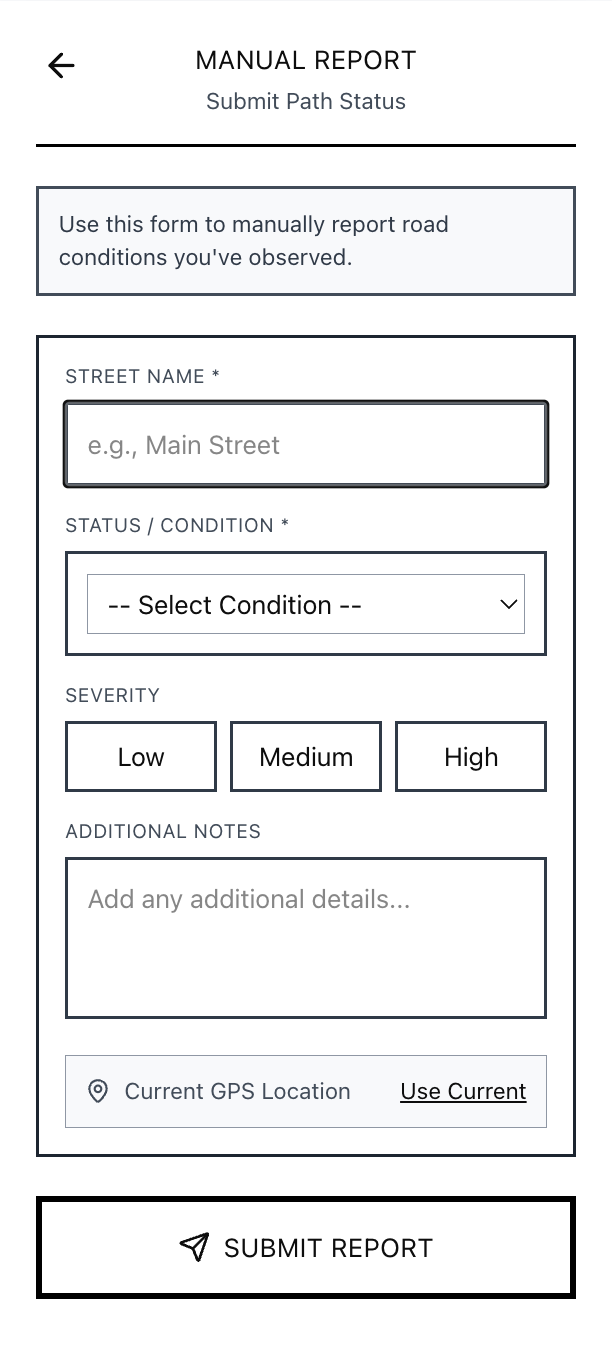
\includegraphics[height=0.7\textheight, keepaspectratio]{Images/RV_SRC/BBP_UI/manualtrip.png}
    \caption{Mockup of the BBP Manual Reporting UI}
    \label{fig:manual_report}
\end{figure}

\par The Manual Report interface corresponds to the "Manual Mode" defined in the system requirements, enabling users to contribute to the bike path inventory without recording a full trip. This form is designed for the precise insertion of publishable information regarding specific road segments.

\par The core of the interface is a structured form requiring the user to identify the "Street Name," satisfying the requirement to specify the location of the path manually. Below this, the "Status / Condition" dropdown allows the user to categorize the quality of the path (e.g., optimal, requires maintenance), while the "Severity" toggle (Low, Medium, High) provides granular detail on any reported obstacles. A text area for "Additional Notes" permits the inclusion of qualitative descriptions that may not fit into predefined categories.

\par To enhance usability, the interface includes a "Current GPS Location" feature, allowing users to quickly populate the location field using their device's current coordinates. Once the form is complete, the "Submit Report" button finalizes the entry, making the data available for the system to process and potentially merge with other user reports.

\subsection{Trip Details and Publication}
\label{sect:trip_details}

\begin{figure}[H]
    \centering
    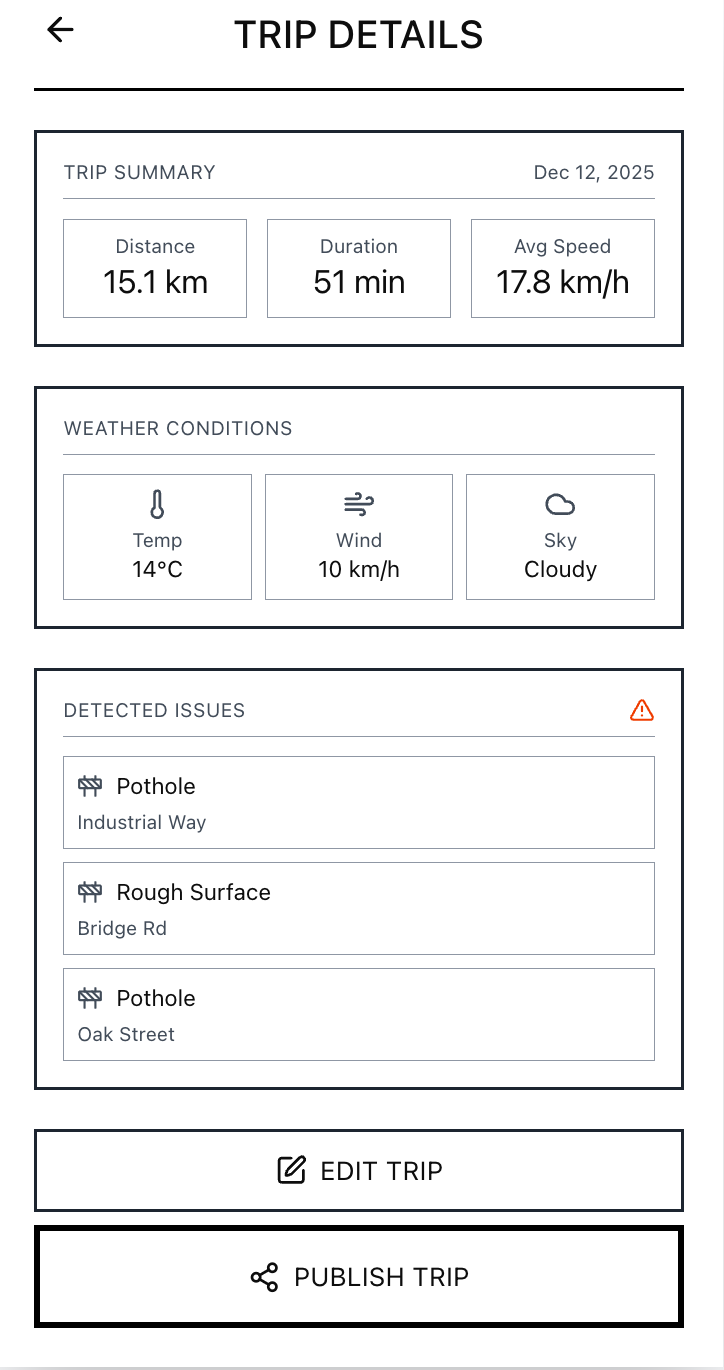
\includegraphics[height=0.6\textheight, keepaspectratio]{Images/RV_SRC/BBP_UI/recenttripdetails.png}
    \caption{Mockup of the BBP Trip Details and Publication UI}
    \label{fig:trip_details}
\end{figure}

\par Accessing a specific entry from the "Recent Trips" list on the homepage directs the user to the Trip Details interface. This view acts as a permanent record of the user's cycling activity, displaying the stored "Trip Summary" statistics (distance, duration, and average speed) alongside the historical "Weather Conditions" captured at the time of the ride.

\par Crucially, this interface serves as the final review stage before data sharing. The "Detected Issues" section lists the road anomalies (e.g., potholes, rough surfaces) that were confirmed during the recording phase or manually inserted. Users can review these details to ensure accuracy. The interface provides two primary actions: "Edit Trip," which allows for the retrospective modification of data (e.g., correcting a street name or adjusting issue severity), and "Publish Trip." Selecting "Publish Trip" changes the visibility of the data from private to public, thereby fulfilling the system requirement to make path status information available to the wider community for route calculation and merging.

\subsection{Edit Trip Interface}
\label{sect:edit_trip}

\begin{figure}[H]
    \centering
    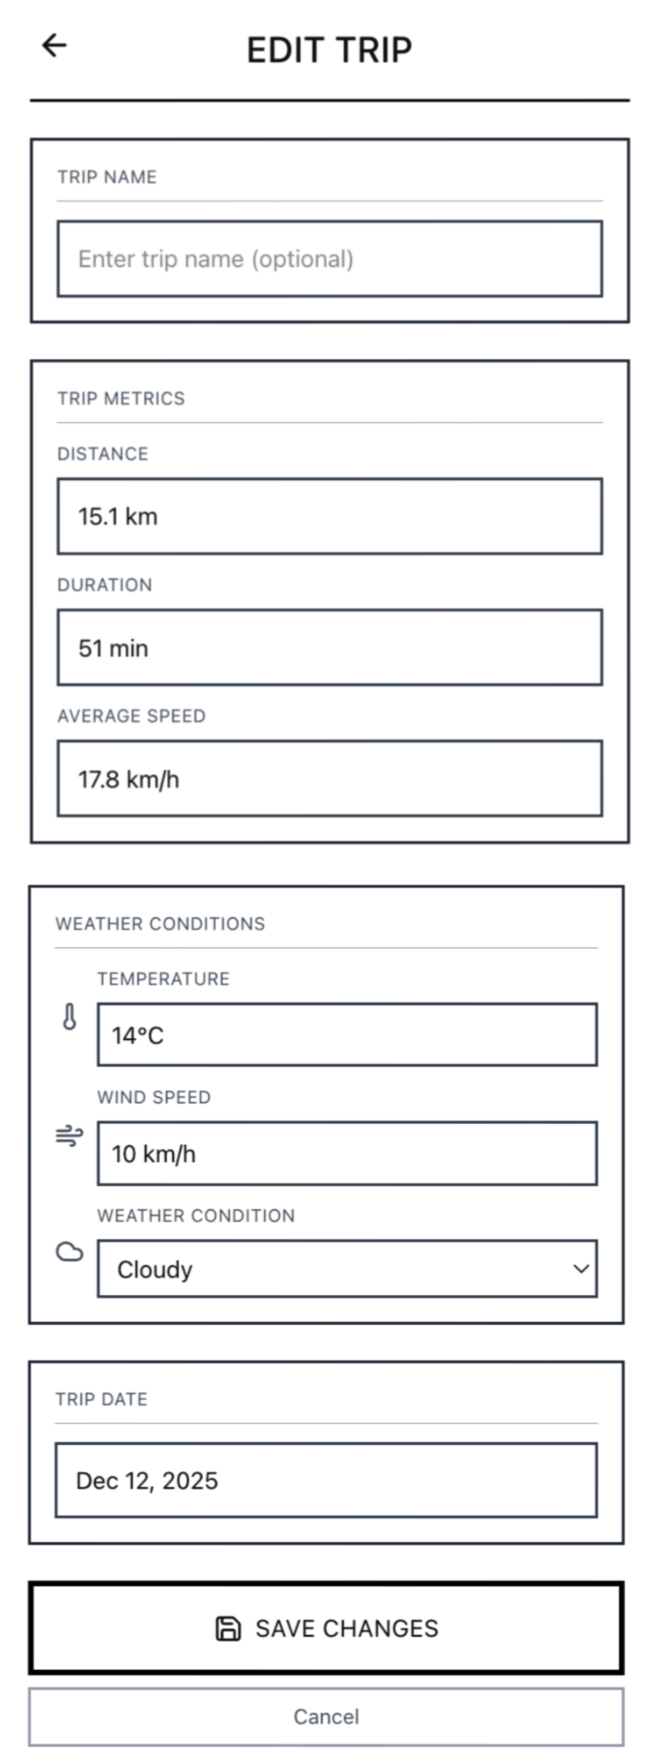
\includegraphics[height=0.9\textheight, keepaspectratio]{Images/RV_SRC/BBP_UI/editrecenttrip.png}
    \caption{Mockup of the BBP Edit Trip UI}
    \label{fig:edit_trip}
\end{figure}

\par Initiated by selecting the "Edit Trip" action from the Trip Details view, this interface empowers the user to refine the data associated with a specific cycling activity. This functionality is essential for addressing the system requirement that allows users to correct information acquired by BBP before it is finalized or published.

\par The form is organized into modular sections. The "Trip Name" field allows users to assign a personal identifier to the route. Below this, the "Trip Metrics" section (Distance, Duration, Average Speed) and "Trip Date" are presented in editable fields, enabling the user to manually adjust values in case of GPS drift or sensor errors during the recording phase. Furthermore, the "Weather Conditions" section permits the modification of meteorological data such as temperature, wind speed, and general conditions (e.g., changing "Sunny" to "Cloudy"), ensuring that the context of the trip remains accurate even if the external weather service provided mismatched local data. The process is concluded by clicking "Save Changes," which updates the local record and prepares the validated data for potential publication.


\subsection{Trip Publication Confirmation}
\label{sect:trip_publish_name}

\begin{figure}[H]
    \centering
    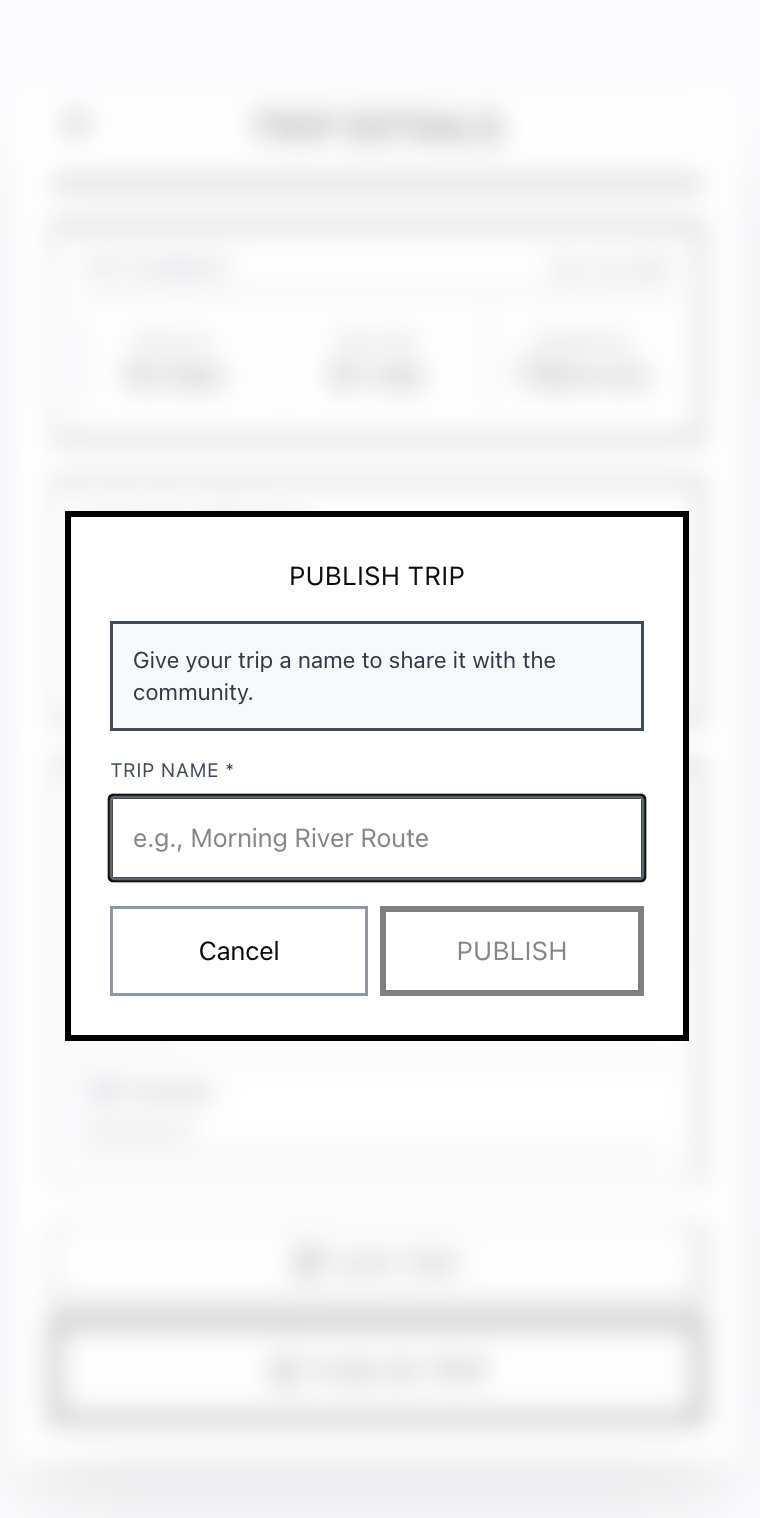
\includegraphics[height=0.45\textheight, keepaspectratio]{Images/RV_SRC/BBP_UI/tripname.png}
    \caption{Mockup of the BBP Trip Publication Name Dialog}
    \label{fig:trip_publish_name}
\end{figure}

\par This modal interface appears as an overlay immediately after the user selects "Publish Trip" from the details view. It represents the final confirmation step required to transition the trip data from a private record to a shared community asset.

\par To ensure that published routes are identifiable and searchable by other users, the system mandates the assignment of a "Trip Name". The user is presented with a required text field to provide a descriptive title (e.g., "Morning River Route"). This step ensures that when the data is merged into the global bike path inventory, it carries a meaningful identifier. Clicking the primary "PUBLISH" button commits the transaction, making the path status and obstacle data available to the BBP community for future route planning and statistical aggregation.


\subsection{Publication Confirmation}
\label{sect:publication_confirm}

\begin{figure}[H]
    \centering
    \begin{minipage}[b]{0.48\textwidth}
        \centering
        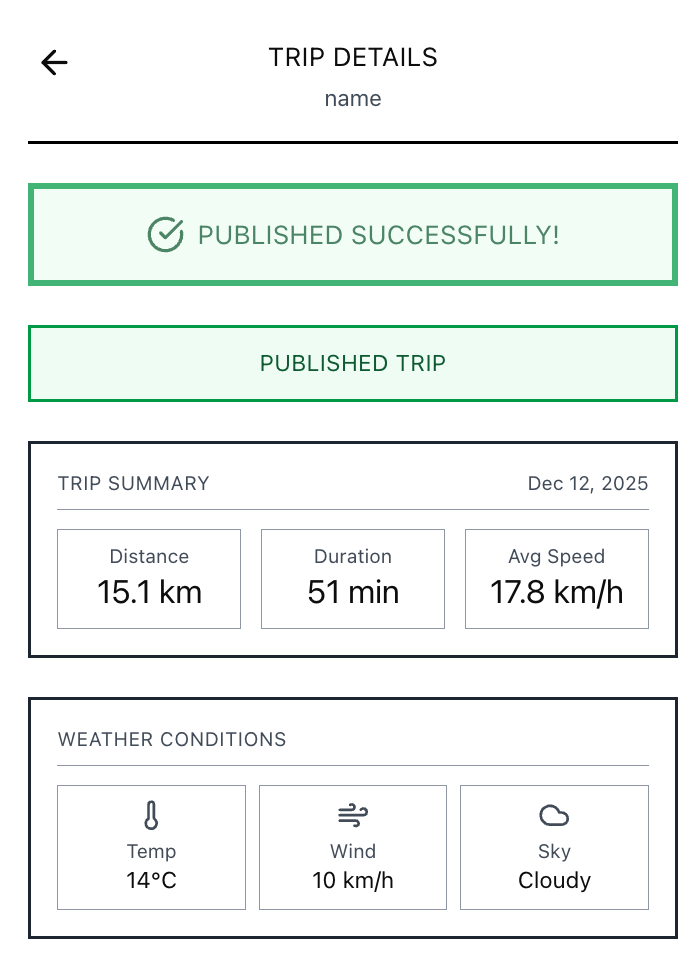
\includegraphics[height=0.3\textheight, keepaspectratio]{Images/RV_SRC/BBP_UI/publishedtrippopup.png}
        \caption{Success Feedback}
        \label{fig:publish_popup}
    \end{minipage}
    \hfill
    \begin{minipage}[b]{0.48\textwidth}
        \centering
        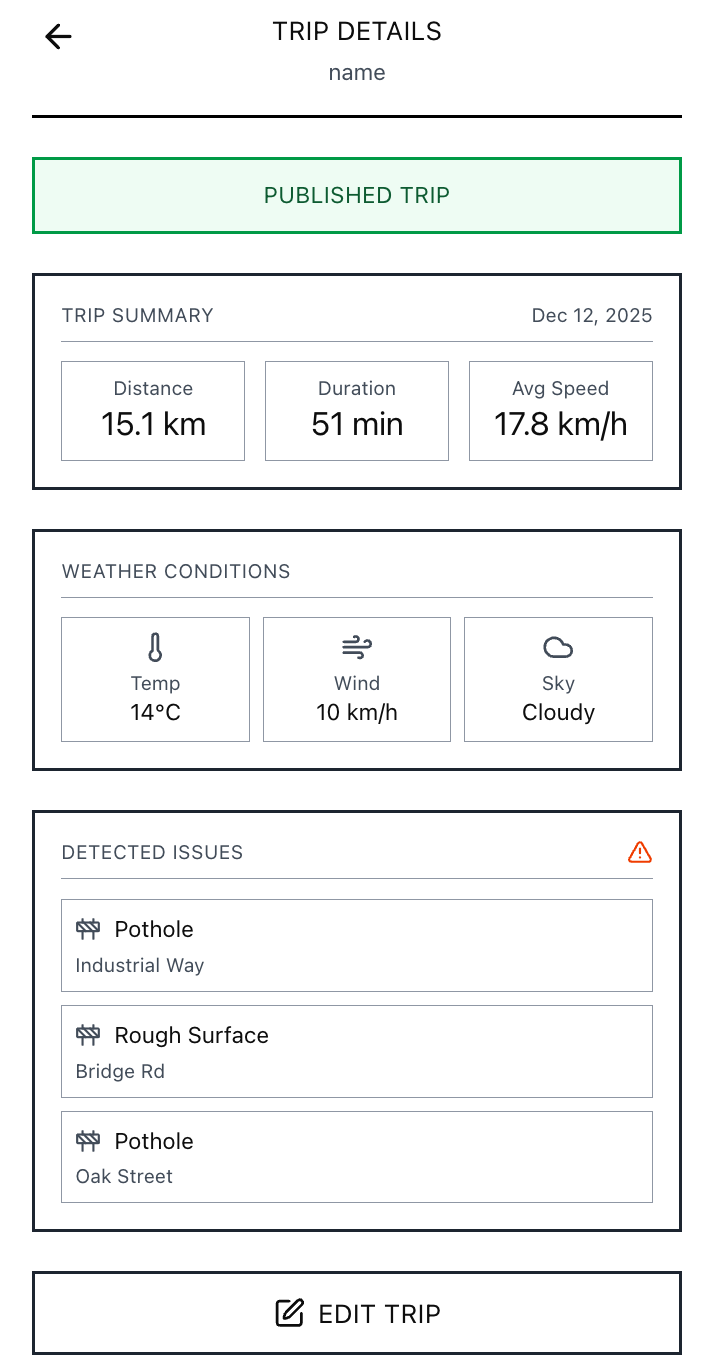
\includegraphics[height=0.5\textheight, keepaspectratio]{Images/RV_SRC/BBP_UI/publishedtrip.png}
        \caption{Permanent Published State}
        \label{fig:publish_state}
    \end{minipage}
    \caption{Trip Publication Workflow Results}
    \label{fig:trip_published_flow}
\end{figure}

\par Once the user confirms the trip name, the system executes the publication process. As shown in Figure \ref{fig:publish_popup}, the interface provides immediate visual feedback via a transient "Published Successfully!" notification banner at the top of the screen. This confirms to the user that their data has been successfully transmitted to the server and merged with the global inventory.

\par Following this confirmation, the Trip Details view updates to reflect the new visibility status of the record. As depicted in Figure \ref{fig:publish_state}, a permanent green "Published Trip" indicator replaces the previous action buttons. This visual cue signifies that the path status and obstacle data are now public and accessible to the community. The user retains access to the trip statistics and weather data, but the record is now locked as a shared contribution.

\subsection{Map and Navigation Interface}
\label{sect:map_nav}

\begin{figure}[H]
    \centering
    % Left image: The main map view
    \begin{minipage}[b]{0.48\textwidth}
        \centering
        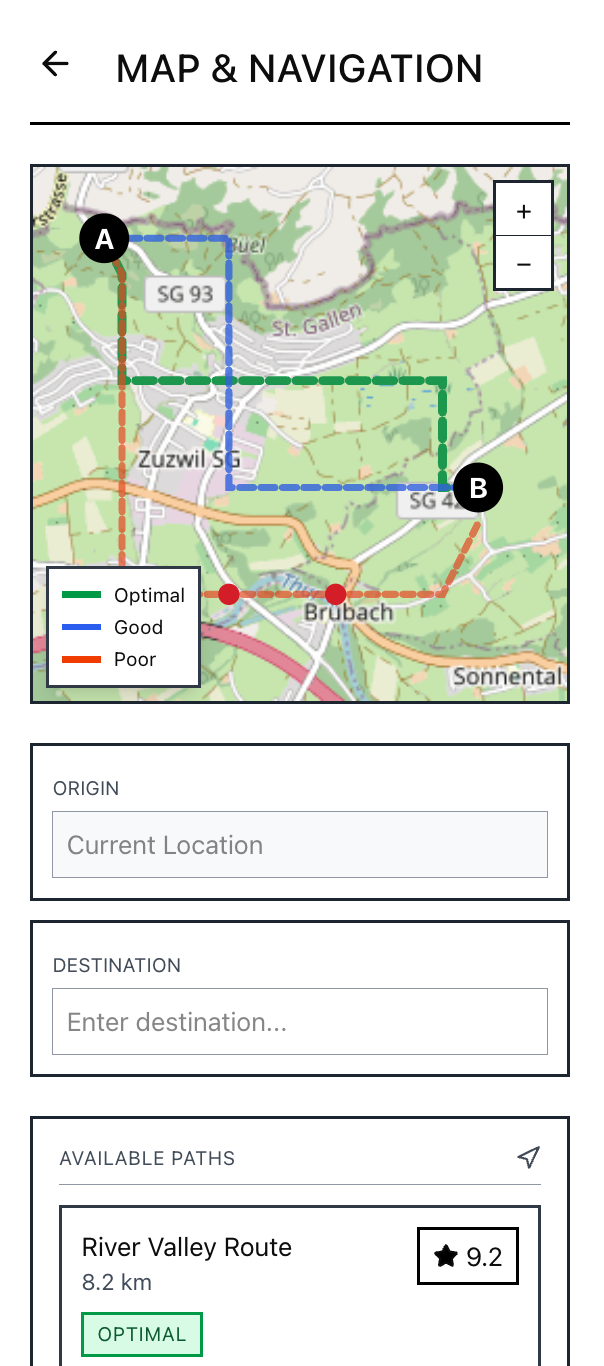
\includegraphics[height=0.45\textheight, keepaspectratio]{Images/RV_SRC/BBP_UI/findtrip.png}
        \caption{Map Visualization}
        \label{fig:map_view}
    \end{minipage}
    \hfill
    % Right image: The list details
    \begin{minipage}[b]{0.48\textwidth}
        \centering
        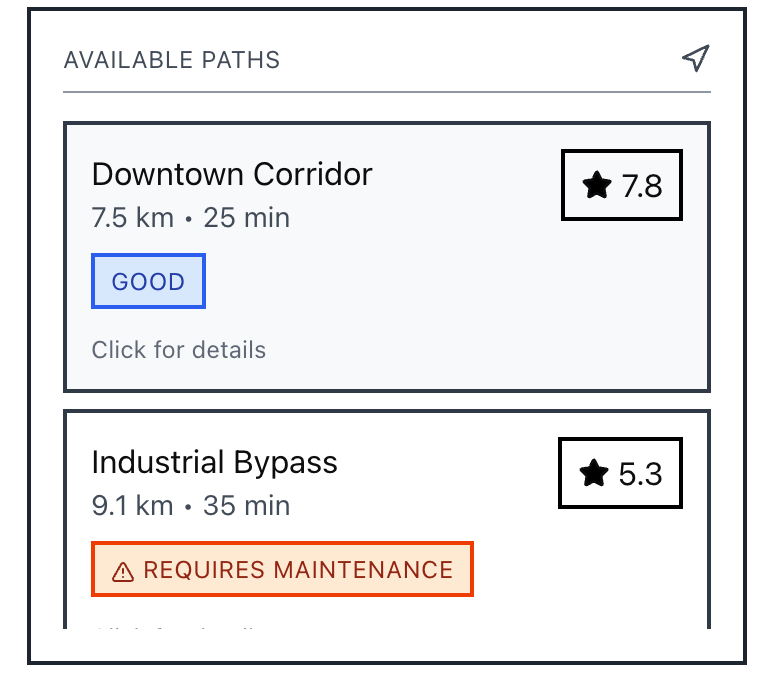
\includegraphics[width=\textwidth, keepaspectratio]{Images/RV_SRC/BBP_UI/availabletripfrommap.png}
        \caption{Path Selection List}
        \label{fig:path_list}
    \end{minipage}
    \caption{BBP Map Navigation and Path Selection UI}
    \label{fig:map_navigation_full}
\end{figure}

\par Accessible via the "Search Trip" action on the homepage, the Map \& Navigation interface serves the primary consumer goal of the BBP system: allowing users to find the best routes based on community data. The interface is driven by two primary input fields, "Origin" and "Destination," allowing users to query paths between specific points.

\par The central visual component (Figure \ref{fig:map_view}) is the interactive map, which renders the available routes color-coded by quality (Green for "Optimal," Blue for "Good," and Orange for "Poor"). This visualization directly reflects the aggregated status information provided by other users.

\par As shown in Figure \ref{fig:path_list}, the "Available Paths" section lists the specific route options ranked by a calculated "Score". For example, a path marked "Requires Maintenance" appears with a lower score (e.g., 5.3), alerting the user to potential issues. By clicking on a specific result in this list, the user can access expanded details, such as specific obstacle reports, and explicitly select the trip to commence navigation.


\subsection{Guest Access Interface}
\label{sect:guest_access}

\begin{figure}[H]
    \centering
    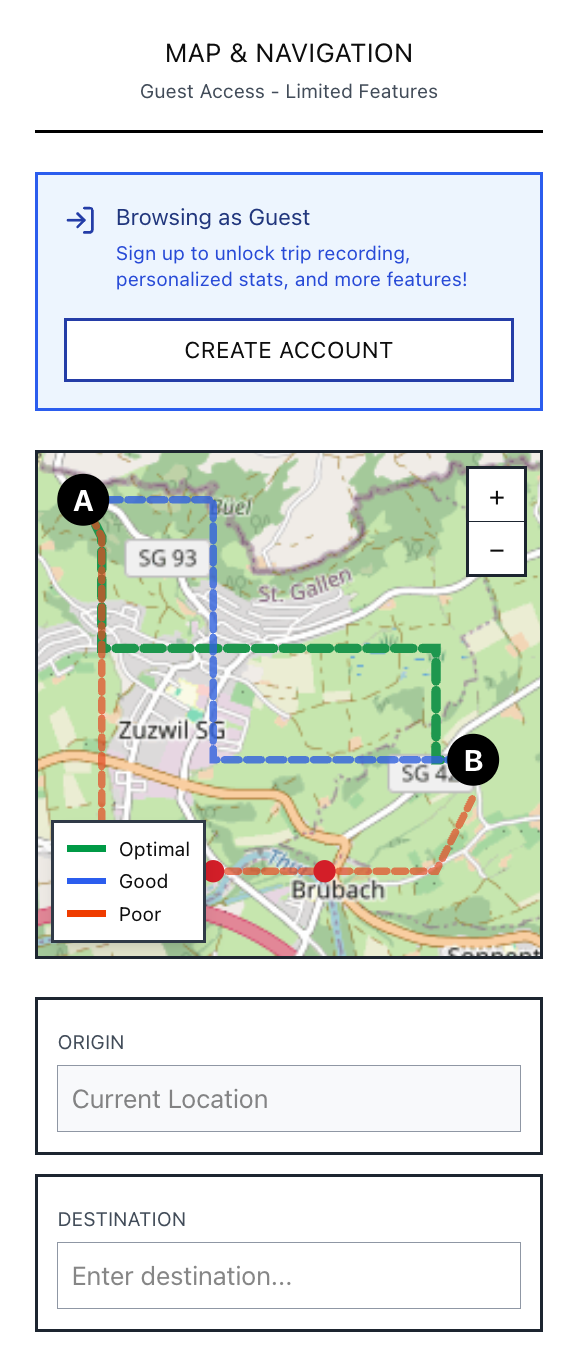
\includegraphics[height=0.9\textheight, keepaspectratio]{Images/RV_SRC/BBP_UI/guestaccess.png}
    \caption{Mockup of the BBP Guest Access UI}
    \label{fig:guest_access}
\end{figure}

\par The Guest Access interface represents the system's state when accessed by an unregistered user or a user who has chosen to "Continue as Guest" from the login screen. This design fulfills the critical requirement that "Any user, either registered or not, can take advantage of the information collected by BBP."

\par As shown in the mockup, the core "Map \& Navigation" functionality remains fully accessible, allowing the user to input an Origin and Destination to search for bike paths. The visualization of path status (Optimal, Good, Poor) is identical to the registered view, ensuring safety information is public.

\par However, distinct UI elements clarify the limitations of this mode. A prominent banner at the top explicitly identifies the session as "Browsing as Guest" and includes a call-to-action "Create Account" button. This banner informs the user that advanced features, specifically trip recording, personalized statistics, and contributing data, are locked, thereby encouraging conversion to a registered account without blocking access to the essential utility of the application.

\subsection{Conclusions}
\label{sect:ui_conclusions}

\par The user interface designs presented in this chapter demonstrate a comprehensive coverage of the functional requirements defined for the Best Bike Paths (BBP) system. The proposed visual hierarchy effectively distinguishes between the two primary user roles: enabling registered cyclists to actively contribute data through the \textit{Automated} and \textit{Manual} acquisition modes, while ensuring that unregistered guests have seamless access to the resulting community inventory, as mandated by the system specifications.

\par A key focus of the interface design is data integrity. The specific workflows for \textit{Trip Completion} and \textit{Trip Editing} introduce necessary human-in-the-loop verification steps, forcing users to validate sensor-detected anomalies before data is finalized. This design directly addresses the requirement to filter false positives from automated sources.

\par Finally, the transition from individual contribution to collective utility is visualized through the \textit{Publication} and \textit{Path Selection} screens. By explicitly separating private tracking from public sharing, the UI supports the system's goal of aggregating disparate user reports into a cohesive, scored, and reliable map for safe route planning.